\documentclass{article}
\usepackage{graphicx}
\topmargin=0.0in %length of margin at the top of the page (1 inch added by default)
\oddsidemargin=0.0in %length of margin on sides for odd pages
\evensidemargin=0in %length of margin on sides for even pages
\textwidth=6.5in %How wide you want your text to be
\marginparwidth=0.5in
\headheight=0pt %1in margins at top and bottom (1 inch is added to this value by default)
\headsep=0pt %Increase to increase white space in between headers and the top of the page
\textheight=9.0in %How tall the text body is allowed to be on each page
\newcommand\tab[1][3cm]{\hspace*{#1}}
 \begin{document}
 	\begin{center}
 		{
 			\huge \textbf{ Calculations for deciding the components to be used for drone(quadcopter)}
 		}
 	\end{center}
 	\begin{flushleft}
 	\vspace{0.5in}
 	\large
 	
 \textbf{\underline{	First, calculate the approx weight of whole quadcopter}}
 	\begin{enumerate}
 		\item	Weight of frame 	 =	  300 gm
 		\item Weight of bettary	 = 	  600 gm
 		\item BLDC Motors 	= 	  4x85 gm
 		\item 	 Propellers 		= 	  4x15 gm
 		\item	Esc + R pi + FC(apm)= 	  200 gm
	 	\item	Camara + gimble 	= 	  300 gm
 		\item	Buffer weight	=           200 gm
		\hrule
 		
 	\end{enumerate}
 \hspace{0.2in}	total weight = \textbf{2000 gm}  \newline
	 \\
 	As per calculation,the  total weight of drone is 2 kg about.\newline
 	
 	 So you need to generate 3 times of thrust of its weight for smooth lifting the quad and hovering.\newline
 	 
 	So we need to generate 6 kg of thrust from four motors.\newline
 	
 	So each motor needs to generate 1.5 kg of thrust.\newline
 	
 	Now according to required thrust we have to choose specified motors and propellers\newline
 	
 	First of all, calculate the power.\\
 	Equation for power is 
 	
 \end{flushleft}
 \begin{center}
 	
 	\mathbf {\[ Power = propller’s constant * (R.P.M.)^{power factor} \]}
 \end{center}
 \large
 Now thrust is,
 \begin{center}
 
 		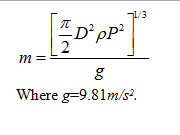
\includegraphics{eq1}
 \end{center}
 \begin{flushleft}
 	D= diameter of propeller \\
 	 &\X\rho     = Air constant 1.22\\
 	P= power supplied by motor to propeller\newline
 	
 	 Now calculate the power according to your propeller’s constant and put it in equation 2.\newline
 	
 	Do the propeller test and get the readings, you can also find the prop test reading from sellers. \newline
 	
 	we choose \textbf{10x4E} propeller. We got power \textbf{222W – 15 A.}
 	By putting the all the values in equation 2. We  get 1.6 kg of thrust per motor.
 	\textbf{1.6*4 = 6.4kg} Which is enough to lift 2 kg of the quadcopter.\newline
 	\newline
 	
 
 		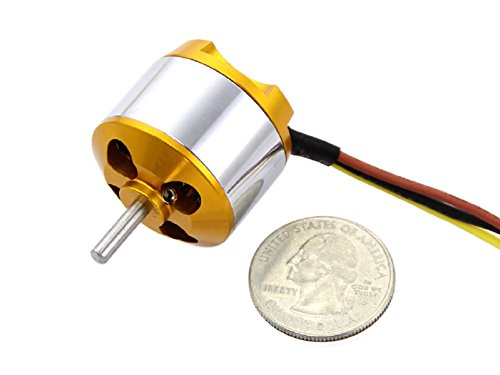
\includegraphics[width = 200 px]{motor}
 	
 	
 \end{flushleft}
\end{document}
 		